%%%%Use this as a filler to get the template working
%%Introduction
\chapter{Di-Higgs Production}
\label{chap:dihiggs}
Measuring di-Higgs production is necessary to further confirm the SM or find evidence for beyond the SM physics. The small SM production rate makes the channel an important place to look for new physics.  In particular, the di-Higgs production rate gives a handle to more accurately measure the Higgs potential.  This dissertation looks at both the measurement of the SM di-Higgs production rate and to search for new physics through resonant di-Higgs production. 
\section{Standard Model}
The Higgs self coupling potential in the SM is
\begin{equation}
V_{\mathrm{self-coupling}} = \lambda(|\Phi^{\dagger}\Phi|)^{2}
\end{equation}
When ${\Phi}$ is expanded around the VeV, $v$, the self coupling term can be written as
\begin{equation}
V_{\mathrm{self-coupling}} \supset \lambda v H^{3} + \frac{\lambda}{4}H^{4}
\end{equation}
where the first term, ${\lambda v H^{3}}$ is the coupling between three Higgs bosons with strength ${\lambda v \equiv \lambda_{HHH}}$\cite{Belusevic:2004pz}. The trilinear Higgs coupling can be probed at the LHC by measuring the cross section of events with two Higgs Bosons in the final state.\newline



\indent  Currently at the LHC, there are two dominant ways to produce di-Higgs events, the trilinear Higgs coupling gluon-gluon fusion (ggF) diagram and a box diagram, figure ~\ref{fig:dihiggs}. These diagrams interfere destructively, resulting in a SM prediction for the cross section, 
\begin{equation}
\sigma_{\mathrm{HH}} = 33.53\mathrm{fb}^{+4.3\%}_{-6.0\%}(\mathrm{QCD \ unc.})\pm{5.9\%} \mathrm{(other \ unc.)} 
\end{equation}
in pp collisions at 13 TeV \cite{Sirunyan:2018two}. This makes the trilinear coupling extremely hard to measure at the LHC. Additionally, since the cross section is so small, it is an promising place to look for deviations from the SM, since any enhancement to the cross section would be indicative of new physics.

\begin{figure}[h]
\footnotesize
\begin{center}
\begin{tikzpicture}
\begin{feynman}
\vertex (i1);
\vertex [right = of i1] (t1);
\vertex [dot][below right =of t1] (t3);
\vertex [below left= of t3] (t2);
\vertex [left = of t2] (i2);
\vertex [right =of t3][dot](h){};
\vertex [above right = of h] (f1){\(H\)};
\vertex [below right = of h] (f2){\(H\)};
\diagram* {
(i1) -- [gluon] (t1),
(i2) -- [gluon] (t2),
(t1) -- [fermion](t3) -- [fermion] (t2) -- [fermion,edge label'=\(t/b\)](t1),
(t3) -- [scalar,edge label'=\(H^{*}\)] (h),
(f1) -- [scalar] (h) -- [scalar](f2)
};
\vertex [right=0.75cm of h] {\(\lambda_{HHH}\)};
\end{feynman}
\end{tikzpicture}
\hspace{1cm}
\begin{tikzpicture}
\begin{feynman}
\vertex (i1);
\vertex [ right = of i1] (t1);
\vertex [right = of t1] (t2);
\vertex [below = of t2] (t3);
\vertex [left = of t3] (t4);
\vertex [ left=of t4] (i2);
\vertex [ right =of t2] (f1){\(H\)};
\vertex [ right=of t3] (f2){\(H\)};
\diagram* {
(i1) -- [gluon] (t1),
(i2) -- [gluon] (t4),
(t1) -- [fermion](t2) -- [fermion] (t3) -- [fermion](t4) -- [fermion,edge label'=\(t/b\)] (t1),
(t2) -- [scalar] (f1),
(t3) -- [scalar] (f2)
};
\end{feynman}
\end{tikzpicture}
\caption[Di-Higgs production diagrams]{The dominate production method for di-Higgs events at the LHC with ${\sqrt{s} = 13 \mathrm{TeV}}$, with the trilinear Higgs coupling on the left}
\end{center}
\end{figure}
\label{fig:dihiggs}

\indent The SM di-Higgs production is a continuum production, with a turn-on at two times the Higgs mass, 250 GeV. Figure ~\ref{fig:SM_cont} shows the continuum distribution, as expected, it is a falling power law distribution peaked around 400 GeV. 

\begin{figure}[h]
\begin{center}
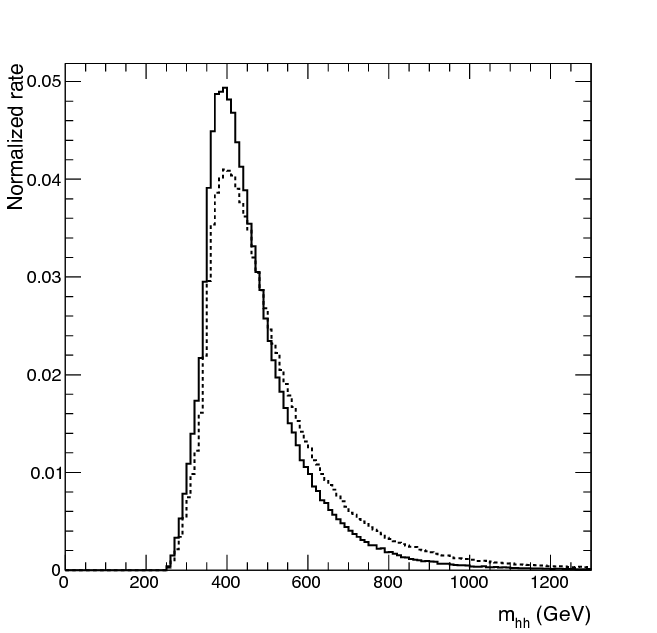
\includegraphics[scale=0.3]{figures/SM_continuum}
\caption[Normalized di-Higgs cross section]{Normalized differential cross section for pp ${\rightarrow}$ hh in the SM as a function of the invariant mass of the two Higgs bosons. The solid and dotted lines correspond respectively to ${\sqrt{s} = 14 \textrm{ and } 100}$ TeV.\cite{azatov:2015}}
\label{fig:SM_cont}
\end{center}
\end{figure}


\section{Resonant Production}
There are several BSM models that may enhance the rate of di-Higgs production at the LHC. This section will give an overview of a few of these models
\subsection{Complex Higgs Singlet}
The addition of a complex scalar singlet to the SM results in three neutral scalar particles after spontaneous symmetry breaking, which mix to give mass eigenstates, including the observed 125 GeV scalar \cite{PhysRevD.97.015022}.\newline
The normalizable scalar potential is
\begin{equation}
\begin{split}
V(\Phi,S_{c}) = \frac{\mu^{2}}{2}\Phi^{\dagger}\Phi + \frac{\lambda}{4}(\Phi^{\dagger}\Phi)^{2} \\
+ (\frac{1}{4}\delta_{1}\Phi^{\dagger}\Phi{}S_{c} + \frac{1}{4}\delta_{3}\Phi^{\dagger}\Phi{}S_{c}^{2} \\
+ a_{1}S_{c} + \frac{1}{4}b_{1}S_{c}^{2} + \frac{1}{6}e_{1}S_{c}^{3} + \frac{1}{6}e_{2}S_{c}|S_{c}|^{2} \\
+ \frac{1}{8}d_{1}S^{4} + \frac{1}{8}d_{3}S_{c}^{2}|S_{c}|^{2} + \mathrm{H.C.}) \\
+ \frac{1}{4}d_{2}(|S_{2}|^{2})^{2} + \frac{\delta_{2}}{2}\Phi^{\dagger}\Phi|S_{c}|^{2} + \frac{1}{2}b_{2}|S_{c}|^{2}
\end{split}
\end{equation}
\indent After spontaneous symmetry breaking, the fields are defined as:
\begin{equation}
\Phi = \binom{0}{\frac{h+v}{\sqrt{2}}}; S_{c} = \frac{1}{\sqrt{2}}(S+v_{s} + i(A + v_{A})).
\end{equation}
$v_{A}$ is set to 0 to conserve CP symmetry.\newline
The mass eigenstate fields are given by:
\begin{equation}
\begin{pmatrix}
h_{1}\\
h_{2}\\
h_{3}
\end{pmatrix}
= \begin{pmatrix}
c_{1} & -s_{1} & 0\\
s_{1}c_{2} & c_{1}c_{2} & s_{2}\\
s_{1}s_{2} & c_{1}s_{2} & -c_{2}
\end{pmatrix} 
\begin{pmatrix}
h\\
S\\
A\\
\end{pmatrix}
\end{equation}
where ${c_{i} = \cos{\theta_{i}}}$, h is the SU(2) doublet field, and S and A are the real and imaginary components of the complex scalar ${S_{c}}$.
Assigning the SM-like Higgs boson as ${h_{1}}$ with ${m_{1} = 125 GeV}$  and ${v = 246 GeV}$,  ${h_{2}}$ and ${h_{3}}$ are physical heavy Higgs bosons with ${m_{2}, m_{3} > m_{1}}$. The coupling of ${h_{1}}$ to SM particles is dominant, suppressed by a factor of ${c_{1}}$ from the SM rate, with the ${h_{2}}$ couplings suppressed by ${s_{1}c_{2}}$ and ${h_{3}}$ couplings suppressed by ${s_{1}s_{2}}$. ATLAS has set limits on ${c_{1} > 0.94}$ at 95\% CL in RUN-1. As the ${h_{1}}$ couplings become more SM-like (${\theta_{1}\rightarrow{0}}$), the allowed ${h_{2}}$ couplings become suppressed.\newline

\begin{figure}[h]
\begin{center}
\begin{tikzpicture}
\begin{feynman}
\vertex (i1);
\vertex [right = of i1] (t1);
\vertex [dot][below right =of t1] (t3);
\vertex [below left= of t3] (t2);
\vertex [left = of t2] (i2);
\vertex [right =of t3][dot](h){};
\vertex [above right = of h] (f1){\(h_{j}\)};
\vertex [below right = of h] (f2){\(h_{k}\)};
\diagram* {
(i1) -- [gluon] (t1),
(i2) -- [gluon] (t2),
(t1) -- [fermion](t3) -- [fermion] (t2) -- [fermion](t1),
(t3) -- [scalar,edge label'=\(h_{i}\)] (h),
(f1) -- [scalar] (h) -- [scalar](f2)
};
\end{feynman}
\end{tikzpicture}
\hspace{1cm}
\begin{tikzpicture}
\begin{feynman}
\vertex (i1);
\vertex [ right = of i1] (t1);
\vertex [right = of t1] (t2);
\vertex [below = of t2] (t3);
\vertex [left = of t3] (t4);
\vertex [ left=of t4] (i2);
\vertex [ right =of t2] (f1){\(h_{j}\)};
\vertex [ right=of t3] (f2){\(h_{k}\)};
\diagram* {
(i1) -- [gluon] (t1),
(i2) -- [gluon] (t4),
(t1) -- [fermion](t2) -- [fermion] (t3) -- [fermion](t4) -- [fermion] (t1),
(t2) -- [scalar] (f1),
(t3) -- [scalar] (f2)
};
\end{feynman}
\end{tikzpicture}
\caption[BSM di-Higgs production diagrams]{Feynman diagrams for the production of ${h_{j}h_{k}}$, ${i, j, k = 1, 2, 3}$.}
\label{fig:FeyComp}
\end{center}
\end{figure}


\indent In the limit of ${\theta_{2}\rightarrow{0}}$, which is in agreement with the single Higgs rates, ${h_{3}}$ does not directly couple to SM fermions or vector bosons. The only way to produce ${h_{3}}$ is through ${h_{1}}$ or ${h_{2}}$, with the largest production rate from ${gg\rightarrow h_{2}\rightarrow h_{1}h_{3}}$, figure ~\ref{fig:FeyComp}. For a range of masses ${m_{2}}$ and ${m_{3}}$ the rate of production of ${h_{1}h_{3} \gg h_{1}h_{1}}$, figure ~\ref{fig:CSH6}. \newline

\begin{figure}[h]
\begin{center}
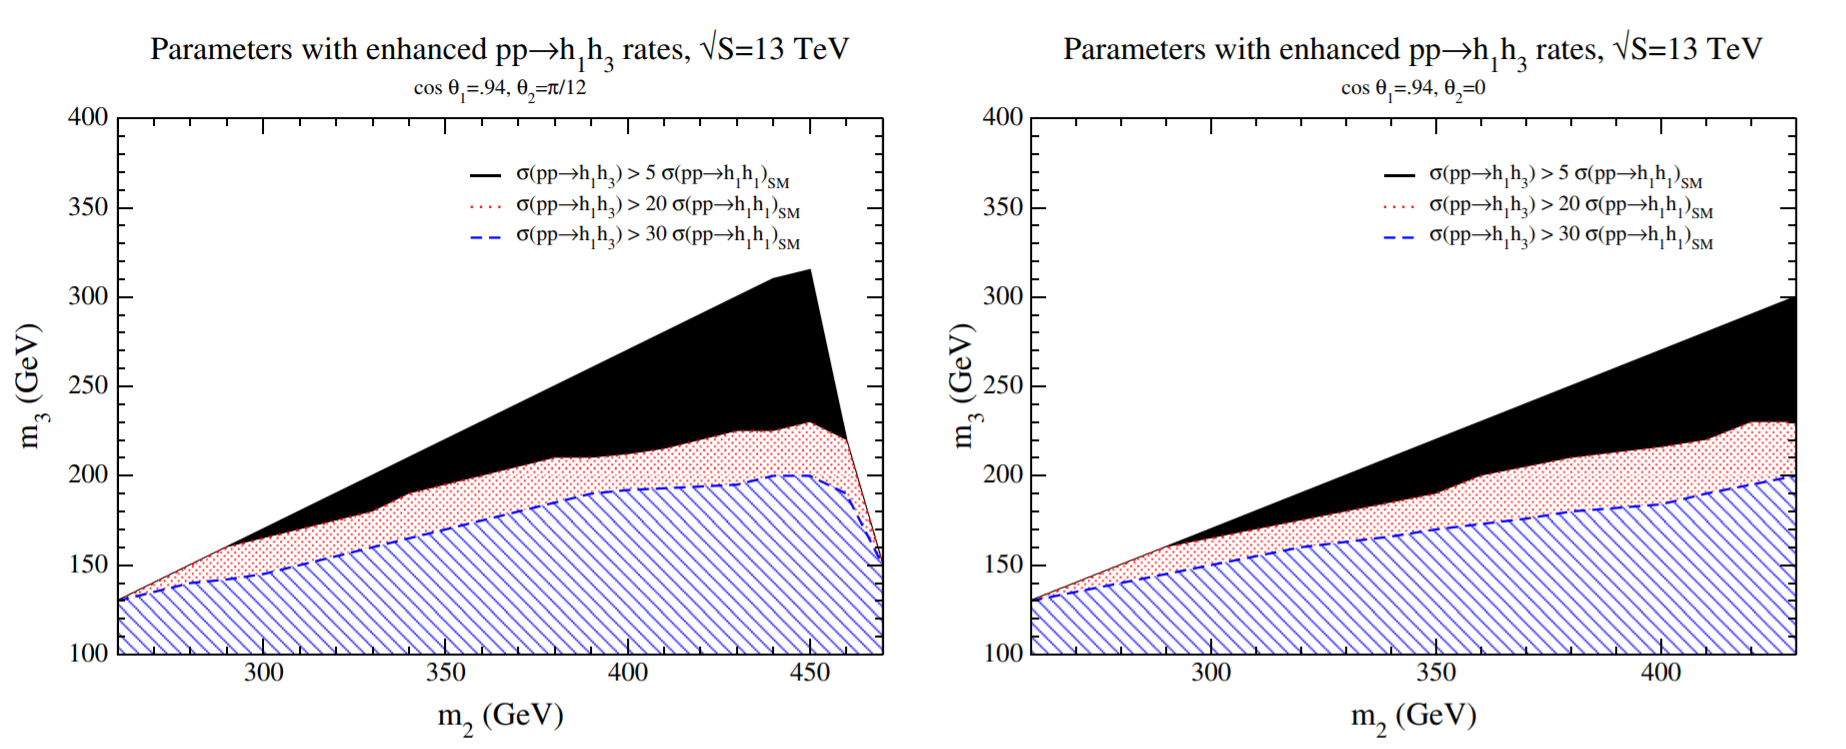
\includegraphics[scale=0.4]{figures/CompHiggsSing_Fig6_2}
\caption[Allowed regions of parameter space with enhanced di-Higgs production]{Regions of parameter space allowed by limits on oblique parameters $S$ $T$ and $U$ from Ref~\cite{deBlas2016}, perturbative unitarity of $2\rightarrow2$ scattering process \cite{PhysRevD.16.1519}, and the minimization of the potential where the rate for ${h_{1}h_{3}}$ production is significantly larger than the SM ${h_{1}h_{1}}$ rate at ${\sqrt{S} = 13 TeV}$.}
\label{fig:CSH6}
\end{center}
\end{figure}


The enhancement can be see in the potential where 
\begin{equation}
V \rightarrow \frac{1}{2}\lambda_{211}h_{1}^{2}h_{2} + \frac{1}{2}\lambda_{311}h_{1}^{2}h_{3} + \frac{1}{2}\lambda_{331}h_{1}h_{3}^{2} + \frac{1}{2}\lambda_{321}h_{1}h_{2}h_{3} + . . .
\label{addhiggs}
\end{equation}
So while the SM trilinear Higgs coupling is determined by ${m_{h}}$, with this extension, the coupling is much less constrained. This leads to enhanced values seen in figure \ref{fig:CHS8}. So while this model would definitely show up in SM di-Higgs production, through the first two terms in equation ~\ref{addhiggs}, a search for one SM Higgs and a heavy Higgs would be more sensitive. This is a promising search moving forward but is not the focus of this dissertation.
\begin{figure}[h]
\begin{center}
\includegraphics[scale=0.65]{figures/CompHiggsSing_Fig8}
\caption[Allowed regions of parameter space with enhanced trilinear coupling]{Region of parameter space allowed by limits on oblique parameters, perturbative unitarity and the minimization of the potential where the ${h_{1}h_{1}h_{1}}$ trilinear coupling is greater than 5 times the SM value.}
\label{fig:CHS8}
\end{center}
\end{figure}

\subsection{Real Higgs Singlet Extension}
One simple explanation of an enhanced di-Higgs production rate at the LHC is the addition of a real scalar Higgs singlet, S \cite{Lewis:2017dme}. In this model, S can only interact with the SM through the Higgs field. In the case where there is no ${Z_{2}}$ symmetry, where ${S\rightarrow -S}$ the scalar field S mixes with the SM Higgs boson. If the mass is large enough, it is possible for S to decay to two on-shell SM Higgs Bosons, significantly enhancing the di-Higgs production rate.\newline
\indent The most general potential that can be added is 
\begin{equation}
V(\Phi,S) = -\mu^{2}\Phi^{\dagger}\Phi + \lambda(\Phi^{\dagger}\Phi)^{2} + \frac{a_{1}}{2}\Phi^{\dagger}\Phi S + \frac{a_{2}}{2}\Phi^{\dagger}\Phi S + b_{1}S + \frac{b_{2}}{2}S^{2} + \frac{b_{3}}{3}S^{3} + \frac{b_{4}}{4}S^{4}.
\end{equation}
Where $\Phi$ is ${\phi_{0} = \frac{(h + v)}{\sqrt{2}}}$ and ${<\phi_{0}> = \frac{v}{2}}$, while ${S = s + x}$ where ${x}$ is the vev of S. By shifting the field, it is possible the set ${x = 0}$. After electroweak symmetry breaking the fields mix to give the two mass eigenstates
\begin{equation}
\binom{h_{1}}{h_{2}} = 
\begin{pmatrix}
\cos{\theta} & \sin{\theta}\\
-\sin{\theta} & \cos{\theta}
\end{pmatrix}
\binom{h}{s}
\end{equation}
With ${m_{1} = 125 GeV}$, the free parameters are ${m_{2}, \theta,a_{2},b_{2}}$ and ${b_{4}}$. For di-Higgs production, in the case of ${m_{2}>2m_{1}}$, the important piece of the potential is 
\begin{equation}
V(h_{1}h_{2}) \supset \frac{\lambda_{111}}{3!}h_{1}^{3} + \frac{\lambda_{211}}{3!}h_{2}h_{1}^{2}
\end{equation}
This give an additional resonant double Higgs production diagram , figure ~\ref{fig:FeyRes}, for ${250 GeV \leq m_{2}}$.
\begin{figure}[h]
\begin{center}
\begin{tikzpicture}
\begin{feynman}
\vertex (i1);
\vertex [right = of i1] (t1);
\vertex [dot][below right =of t1] (t3);
\vertex [below left= of t3] (t2);
\vertex [left = of t2] (i2);
\vertex [right =of t3](h){};
\vertex [above right = of h] (f1){\(h_{1}\)};
\vertex [below right = of h] (f2){\(h_{1}\)};
\diagram* {
(i1) -- [gluon] (t1),
(i2) -- [gluon] (t2),
(t1) -- [fermion](t3) -- [fermion] (t2) -- [fermion](t1),
(t3) -- [scalar,edge label'=\(h_{2}\)] (h),
(f1) -- [scalar] (h) -- [scalar](f2)
};
\end{feynman}
\end{tikzpicture}
\caption[Resonant di-Higgs production diagram]{Feynman diagram for ${h_{2}\rightarrow h_{1}h_{1}}$.}
\label{fig:FeyRes}
\end{center}
\end{figure}

\indent Varying the values of ${b_{4}}$ and ${\sin^{2}{\theta}}$, it is found that the maximum branching ratio (BR) for ${h_{2}\rightarrow h_{1}h_{1}}$ if obtained with ${b_{4} = 4.2, \sin^{2}\theta = 0.12}$. Figure ~\ref{fig:Ian6}, shows the minimum and maximum BR as a function of ${m_{2}}$. The largest BR is when ${m \approx 280 GeV}$ at ${BR(h_{2}\rightarrow h_{1}h_{1}) = 0.76}$. This corresponds to an enhancement in di-Higgs production of approximately 30 times the SM cross section.

\begin{figure}[h]
\begin{center}
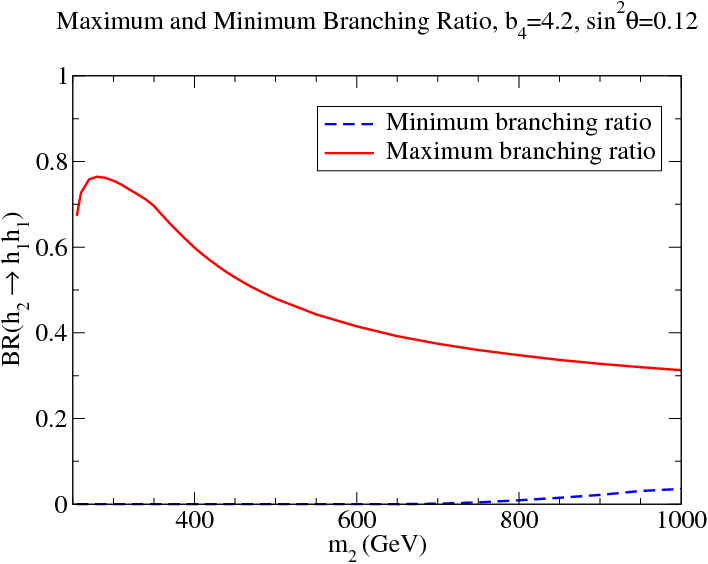
\includegraphics[scale=0.5]{figures/Ian6}
\caption[Allowed branching ratios for resonant di-Higgs production]{Maximum and minimum allowed ${BR(h_{2}\rightarrow h_{1}h_{1})}$ as a function of ${m_{2}}$ for ${b_{4} = 4.2}$ and ${\sin^{2}{\theta} = 0.12}$.}
\label{fig:Ian6}
\end{center}
\end{figure}

\section{Summary}
The SM di-Higgs production rate is an important and achievable measurement for the LHC and HL-LHC. It gives insight to the shape of the Higgs potential through measurement of the trilinear Higgs coupling. It is also a valuable discovery channel for BSM physics, especially for models with an extended Higgs sector, through resonant di-Higgs production. This dissertation will present results for both SM and resonant di-Higgs production.